\protect\hyperlink{main-nav}{≡} \protect\hyperlink{close-nav}{×}

\hypertarget{section-1.3-linear-functions}{%
\section{Section 1.3: Linear
Functions}\label{section-1.3-linear-functions}}

As you hop into a taxicab in Allentown, the meter will immediately read
\$3.30; this is the ``drop'' charge made when the taximeter is
activated. After that initial fee, the taximeter will add \$2.40 for
each mile the taxi drives. In this scenario, the total taxi fare depends
upon the number of miles ridden in the taxi, and we can ask whether it
is possible to model this type of scenario with a function. Using
descriptive variables, we choose \textbackslash{}(m\textbackslash{}) for
miles and \textbackslash{}(C\textbackslash{}) for Cost in dollars as a
function of miles: \textbackslash{}(C(m)\textbackslash{}).

We know for certain that \textbackslash{}(C(0)=3.30\textbackslash{}) ,
since the \$3.30 drop charge is assessed regardless of how many miles
are driven. Since \$2.40 is added for each mile driven, we could write
that if \textbackslash{}(m\textbackslash{}) miles are driven,
\textbackslash{}(C(m)=3.30+2.40m\textbackslash{}) because we start with
a \$3.30 drop fee and then for each mile increase we add \$2.40.

It is good to verify that the units make sense in this equation. The
\$3.30 drop charge is measured in dollars; the \$2.40 charge is measured
in dollars per mile. So
\textbackslash{}{[}C(m)=3.30\textbackslash{}text\{
dollars\}+\textbackslash{}left(2.40\textbackslash{}frac\{\textbackslash{}text\{dollars\}\}\{\textbackslash{}text\{mile\}\}\textbackslash{}right)
(m\textbackslash{}text\{ miles\})\textbackslash{}{]} When dollars per
mile are multiplied by a number of miles, the result is a number of
dollars, matching the units on the 3.30, and matching the desired units
for the C function.

Notice this equation \textbackslash{}(C(m)=3.30+2.40m\textbackslash{})
consisted of two quantities. The first is the fixed \$3.30 charge which
does not change based on the value of the input. The second is the
\$2.40 dollars per mile value, which is a \textbf{rate of change}. In
the equation this rate of change is multiplied by the input value.

Looking at this same problem in table format we can also see the cost
changes by \$2.40 for every 1 mile increase:

\begin{longtable}[]{@{}lllll@{}}
\toprule
\endhead
\textbackslash{}(m\textbackslash{}) & 0 & 1 & 2 & 3\tabularnewline
\textbackslash{}(C(m)\textbackslash{}) & 3.30 & 5.70 & 8.10 &
10.50\tabularnewline
\bottomrule
\end{longtable}

It is important here to note that in this equation, the \textbf{rate of
change is constant}; over any interval, the rate of change is the same.

Graphing this equation,
\textbackslash{}(C(m)=3.30+2.40m\textbackslash{}) we see the shape is a
line, which is how these functions get their name: \textbf{linear
functions}.

\begin{figure}
\centering
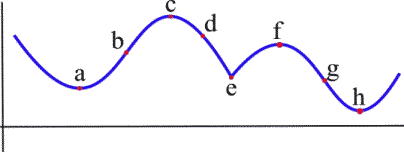
\includegraphics{images/image047.png}
\caption{}
\end{figure}

When the number of miles is zero the cost is \$3.30, giving the point
(0, 3.30) on the graph. This is the vertical or
\textbackslash{}(C(m)\textbackslash{}) intercept. The graph is
increasing in a straight line from left to right because for each mile
the cost goes up by \$2.40; this rate remains consistent.

\hypertarget{linear-function}{%
\paragraph{Linear Function}\label{linear-function}}

A \textbf{linear function} is a function whose graph produces a line.
Linear functions can always be written in the form
\textbackslash{}{[}f(x)=b+mx\textbackslash{}{]} or
\textbackslash{}{[}f(x)=mx+b\textbackslash{}{]} where
\textbackslash{}(b\textbackslash{}) is the initial or starting value of
the function (with input \textbackslash{}(x = 0\textbackslash{})), and
\textbackslash{}(m\textbackslash{}) is the constant rate of change of
the function.

This form of a line is called slope-intercept form of a line.

Many people like to write linear functions in the form
\textbackslash{}(f(x)=b+mx\textbackslash{}) because it corresponds to
the way we tend to speak: "The output starts at
\textbackslash{}(b\textbackslash{}) and increases at a rate of
\textbackslash{}(m\textbackslash{})."

For this reason alone we will use the
\textbackslash{}(f(x)=b+mx\textbackslash{}) form for many of the
examples, but remember they are equivalent and can be written correctly
both ways. {[}While this is the book's convention, in class and in the
videos I will likely use \textbackslash{}(f(x)=mx+b\textbackslash{}).{]}

\hypertarget{slope-and-increasingdecreasing}{%
\paragraph{Slope and
Increasing/Decreasing}\label{slope-and-increasingdecreasing}}

\textbackslash{}(m\textbackslash{}) is the constant rate of change of
the function (also called \textbf{slope}). The slope determines if the
function is an increasing function or a decreasing function.

\begin{itemize}
\tightlist
\item
  \textbackslash{}(f(x)=b+mx\textbackslash{}) is an \textbf{increasing}
  function if \textbackslash{}(m\textbackslash{}gt 0\textbackslash{}).
\item
  \textbackslash{}(f(x)=b+mx\textbackslash{}) is a \textbf{decreasing}
  function if \textbackslash{}(m\textbackslash{}lt 0\textbackslash{}).
\end{itemize}

If \textbackslash{}(m=0\textbackslash{}), the rate of change is 0, and
the function \textbackslash{}(f(x)=b+0x=b\textbackslash{}) is just a
horizontal line passing through the point (0, b), neither increasing nor
decreasing.

To view this video please enable JavaScript, and consider upgrading to a
web browser that \href{http://videojs.com/html5-video-support/}{supports
HTML5 video}

\hypertarget{example-1}{%
\paragraph{Example 1}\label{example-1}}

Marcus currently owns 200 songs in his iTunes collection. Every month,
he adds 15 new songs. Write a formula for the number of songs,
\textbackslash{}(N\textbackslash{}), in his iTunes collection as a
function of the number of months, \textbackslash{}(m\textbackslash{}).
How many songs will he own in a year?

The initial value for this function is 200, since he currently owns 200
songs, so \textbackslash{}(N(0)=200\textbackslash{}). The number of
songs increases by 15 songs per month, so the rate of change is 15 songs
per month. With this information, we can write the
formula:\textbackslash{}{[}N(m)=200+15m.\textbackslash{}{]}

\textbackslash{}(N(m)\textbackslash{}) is an increasing linear function.

With this formula we can predict how many songs he will have in 1 year
(12 months):
\textbackslash{}{[}N(12)=200+15(12)=200+180=380.\textbackslash{}{]}
Marcus will have 380 songs in 12 months.

\hypertarget{calculating-rate-of-change}{%
\paragraph{Calculating Rate of
Change}\label{calculating-rate-of-change}}

Given two values for the input, \textbackslash{}( x\_1 \textbackslash{})
and \textbackslash{}( x\_2 \textbackslash{}), and two corresponding
values for the output, \textbackslash{}( y\_1 \textbackslash{}) and
\textbackslash{}( y\_2 \textbackslash{}), or a set of points,
\textbackslash{}( (x\_1,y\_1) \textbackslash{}) and \textbackslash{}(
(x\_2,y\_2) \textbackslash{}), if we wish to find a linear function that
contains both points we can calculate the rate of change,
\textbackslash{}(m\textbackslash{}):\textbackslash{}{[}m=\textbackslash{}dfrac\{\textbackslash{}text\{change
in output\}\}\{\textbackslash{}text\{change in
input\}\}=\textbackslash{}dfrac\{\textbackslash{}Delta
y\}\{\textbackslash{}Delta
x\}=\textbackslash{}dfrac\{y\_2-y\_1\}\{x\_2-x\_1\}.\textbackslash{}{]}

Rate of change of a linear function is also called the \textbf{slope} of
the line.

Note in function notation,
\textbackslash{}(y\_1=f(x\_1)\textbackslash{}) and
\textbackslash{}(y\_2=f(x\_2)\textbackslash{}), so we could equivalently
write
\textbackslash{}{[}m=\textbackslash{}dfrac\{f(x\_2)-f(x\_1)\}\{x\_2-x\_1\}.\textbackslash{}{]}

To view this video please enable JavaScript, and consider upgrading to a
web browser that \href{http://videojs.com/html5-video-support/}{supports
HTML5 video}

\hypertarget{example-2}{%
\paragraph{Example 2}\label{example-2}}

The population of a city increased from 23,400 to 27,800 between 2002
and 2006. Find the rate of change of the population during this time
span.

The rate of change will relate the change in population to the change in
time. The population increased by 27800-23400=4400 people over the 4
year time interval. To find the rate of change, the number of people per
year the population changed by:
\textbackslash{}{[}\textbackslash{}dfrac\{4400 \textbackslash{}text\{
people\}\}\{4\textbackslash{}text\{
years\}\}=1100\textbackslash{}dfrac\{\textbackslash{}text\{people\}\}\{\textbackslash{}text\{year\}\}=1100
\textbackslash{}text\{ people per year\}.\textbackslash{}{]}

Notice that we knew the population was increasing, so we would expect
our value for \textbackslash{}(m\textbackslash{}) to be positive. This
is a quick way to check to see if your value is reasonable.

\hypertarget{example-3}{%
\paragraph{Example 3}\label{example-3}}

The pressure, \textbackslash{}(P\textbackslash{}), in pounds per square
inch (PSI) on a diver depends upon their depth below the water surface,
\textbackslash{}(d\textbackslash{}), in feet, following the equation
\textbackslash{}(P(d)=14.696+0.43d\textbackslash{}). Interpret the
components of this function.

The rate of change, or slope, 0.434 would have units
\textbackslash{}(\textbackslash{}dfrac\{\textbackslash{}text\{output\}\}\{\textbackslash{}text\{input\}\}=\textbackslash{}dfrac\{\textbackslash{}text\{pressure\}\}\{\textbackslash{}text\{depth\}\}=\textbackslash{}dfrac\{\textbackslash{}text\{PSI\}\}\{\textbackslash{}text\{ft\}\}\textbackslash{})
. This tells us the pressure on the diver increases by 0.434 PSI for
each foot their depth increases.

The initial value, 14.696, will have the same units as the output, so
this tells us that at a depth of 0 feet, the pressure on the diver will
be 14.696 PSI.

We can now find the rate of change given two input-output pairs, and
could write an equation for a linear function if we had the rate of
change and initial value. If we have two input-output pairs and they do
not include the initial value of the function, then we will have to
solve for it.

\hypertarget{example-4}{%
\paragraph{Example 4}\label{example-4}}

Write an equation for the linear function graphed below.

\begin{figure}
\centering
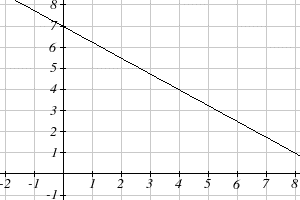
\includegraphics{images/image048.png}
\caption{}
\end{figure}

Looking at the graph, we might notice that it passes through the points
(0, 7) and (4, 4). From the first value, we know the initial value of
the function is b = 7, so in this case we will only need to calculate
the rate of change:
\textbackslash{}{[}m=\textbackslash{}dfrac\{4-7\}\{4-0\}=\textbackslash{}dfrac\{-3\}\{4\}\textbackslash{}{]}

This allows us to write the equation:
\textbackslash{}{[}f(x)=7-\textbackslash{}frac\{3\}\{4\}x\textbackslash{}{]}

\hypertarget{example-5}{%
\paragraph{Example 5}\label{example-5}}

If \textbackslash{}(f(x)\textbackslash{}) is a linear function,
\textbackslash{}(f(3)=-2\textbackslash{}), and
\textbackslash{}(f(8)=1\textbackslash{}), find an equation for the
function.

In Example 3, we computed the rate of change to be
\textbackslash{}(m=\textbackslash{}frac\{3\}\{5\}\textbackslash{}). In
this case, we do not know the initial value
\textbackslash{}(f(0)\textbackslash{}), so we will have to solve for it.
Using the rate of change, we know the equation will have the form
\textbackslash{}(f(x)=b+\textbackslash{}frac\{3\}\{5\}x\textbackslash{}).
Since we know the value of the function when x = 3, we can evaluate the
function at 3:
\textbackslash{}(f(x)=b+\textbackslash{}frac\{3\}\{5\}(3)\textbackslash{}).
Since we know that \textbackslash{}(f(3)=-2\textbackslash{}), we can
substitute on the left side:
\textbackslash{}(-2=b+\textbackslash{}frac\{3\}\{5\}(3)\textbackslash{}).
This leaves us with an equation we can solve for the initial value:
\textbackslash{}(b=-2-\textbackslash{}frac\{9\}\{5\}=-\textbackslash{}frac\{19\}\{5\}\textbackslash{}).

Combining this with the value for the rate of change, we can now write a
formula for this
function:\textbackslash{}{[}f(x)=-\textbackslash{}frac\{19\}\{5\}+\textbackslash{}frac\{3\}\{5\}x.\textbackslash{}{]}

As an alternative to the approach used above to find the initial value,
b, we can use the \textbf{point-slope} form of a line instead.

\hypertarget{point-slope-equation-of-a-line}{%
\paragraph{Point-Slope Equation of a
Line}\label{point-slope-equation-of-a-line}}

An equation for the line passing through the point
\textbackslash{}((x\_1, y\_1)\textbackslash{}) with slope m can be
written as \textbackslash{}{[}y-y\_1=m(x-x\_1)\textbackslash{}{]}

This is called the \textbf{point-slope form of a line}. It is a little
easier to write if you know a point and the slope, but requires a bit of
work to rewrite into slope-intercept form, and requires memorizing
another formula.

To view this video please enable JavaScript, and consider upgrading to a
web browser that \href{http://videojs.com/html5-video-support/}{supports
HTML5 video}

\hypertarget{example-6}{%
\paragraph{Example 6}\label{example-6}}

Working as an insurance salesperson, Ilya earns a base salary and a
commission on each new policy, so Ilya's weekly income,
\textbackslash{}(I\textbackslash{}), depends on the number of new
policies, n, he sells during the week. Last week he sold 3 new policies,
and earned \$760 for the week. The week before, he sold 5 new policies,
and earned \$920. Find an equation for
\textbackslash{}(I(n)\textbackslash{}), and interpret the meaning of the
components of the equation.

The given information gives us two input-output pairs: (3,760) and
(5,920). We start by finding the rate of change:
\textbackslash{}{[}m=\textbackslash{}dfrac\{920-760\}\{5-3\}=\textbackslash{}dfrac\{160\}\{2\}=80.\textbackslash{}{]}

Keeping track of units can help us interpret this quantity. Income
increased by \$160 when the number of policies increased by 2, so the
rate of change is \$80 per policy; Ilya earns a commission of \$80 for
each policy sold during the week.

We can now write the equation using the point-slope form of the line,
using the slope we just found and the point (3,760):
\textbackslash{}{[}I-760= 80(n-3)\textbackslash{}{]}

If we wanted this in function form (slope intercept form), we could
rewrite the equation into that form: \textbackslash{}begin\{align*\}
I-760=\& 80(n-3)\textbackslash{}\textbackslash{} I-760=\&
80n-240\textbackslash{}\textbackslash{} I(n)=\& 520+80n
\textbackslash{}end\{align*\}

This form allows us to see the starting value for the function: 520.
This is Ilya's income when n = 0, which means no new policies are sold.
We can interpret this as Ilya's base salary for the week, which does not
depend upon the number of policies sold.

Our final interpretation is: Ilya's base salary is \$520 per week and he
earns an additional \$80 commission for each policy sold each week.

\hypertarget{graphs-of-linear-functions}{%
\subsection{Graphs of Linear
Functions}\label{graphs-of-linear-functions}}

\hypertarget{graphical-interpretation-of-a-linear-equation}{%
\paragraph{Graphical Interpretation of a Linear
Equation}\label{graphical-interpretation-of-a-linear-equation}}

Graphically, in the equation
\textbackslash{}(f(x)=b+mx\textbackslash{}),

\begin{itemize}
\tightlist
\item
  \textbackslash{}(b\textbackslash{}) is the \textbf{vertical intercept}
  of the graph and tells us we can start our graph at
  \textbackslash{}((0, b)\textbackslash{})
\item
  and \textbackslash{}(m\textbackslash{}) is the \textbf{slope of the
  line} and tells us how far to rise and run to get to the next point.
\end{itemize}

Once we have at least 2 points, we can extend the graph of the line to
the left and right.

\hypertarget{example-7}{%
\paragraph{Example 7}\label{example-7}}

Graph
\textbackslash{}(f(x)=5-\textbackslash{}frac\{2\}\{3\}x\textbackslash{})
using the vertical intercept and slope.

The vertical intercept of the function is (0, 5), giving us a point on
the graph of the line. The slope is
\textbackslash{}(-\textbackslash{}frac\{2\}\{3\}\textbackslash{}). This
tells us that for every 3 units the graph "runs" in the horizontal, the
vertical "rise" decreases by 2 units. In graphing, we can use this by
first plotting our vertical intercept on the graph, then using the slope
to find a second point. From the initial value (0, 5) the slope tells us
that if we move to the right 3, we will move down 2, moving us to the
point (3, 3). We can continue this again to find a third point at (6,
1). Finally, extend the line to the left and right, containing these
points.

\begin{figure}
\centering
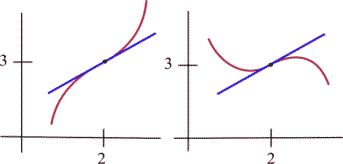
\includegraphics{images/image049.png}
\caption{}
\end{figure}

Another option for graphing is to use transformations of the identity
function \textbackslash{}(f(x)=x\textbackslash{}). In the equation
\textbackslash{}(f(x)=mx\textbackslash{}), the
\textbackslash{}(m\textbackslash{}) is acting as the vertical stretch of
the identity function. When \textbackslash{}(m\textbackslash{}) is
negative, there is also a vertical reflection of the graph. Looking at
some examples will also help show the effect of slope on the shape of
the graph:

\begin{figure}
\centering
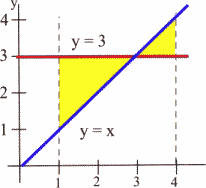
\includegraphics{images/image050.png}
\caption{\textbackslash{}(f(x)=mx\textbackslash{}) for several values of
\textbackslash{}(m\textbackslash{}).}
\end{figure}

In \textbackslash{}(f(x)=mx+b\textbackslash{}), the
\textbackslash{}(b\textbackslash{}) acts as the vertical shift, moving
the graph up and down without affecting the slope of the line. Some
examples:

\begin{figure}
\centering
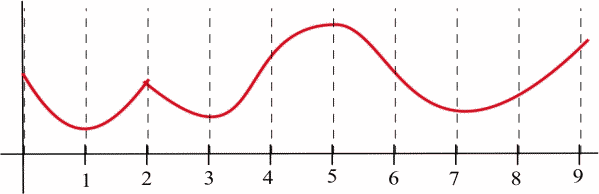
\includegraphics{images/image051.png}
\caption{\textbackslash{}(f(x)=mx+b\textbackslash{}) for several values
of \textbackslash{}(b\textbackslash{}).}
\end{figure}

Try it for yourself using this applet:

\hypertarget{applet_container}{}

\hypertarget{example}{%
\paragraph{Example}\label{example}}

Match each equation with one of the lines in the graph below
\textbackslash{}begin\{align*\} f(x)=\&
2x+3\textbackslash{}\textbackslash{} g(x)=\&
2x-3\textbackslash{}\textbackslash{} h(x)=\&
-2x+3\textbackslash{}\textbackslash{} j(x)=\&
\textbackslash{}frac\{1\}\{2\}x+3 \textbackslash{}end\{align*\}

\begin{figure}
\centering
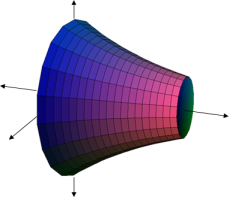
\includegraphics{images/image052.png}
\caption{}
\end{figure}

Only one graph has a vertical intercept of -3, so we can immediately
match that graph with \textbackslash{}(g(x)\textbackslash{}). For the
three graphs with a vertical intercept at 3, only one has a negative
slope, so we can match that line with
\textbackslash{}(h(x)\textbackslash{}). Of the other two, the steeper
line would have a larger slope, so we can match that graph with equation
\textbackslash{}(f(x)\textbackslash{}), and the flatter line with the
equation \textbackslash{}(j(x)\textbackslash{}).

\begin{figure}
\centering
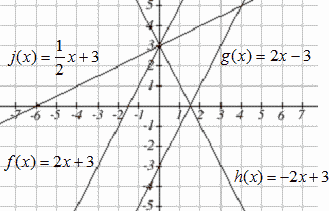
\includegraphics{images/image095.png}
\caption{}
\end{figure}

In addition to understanding the basic behavior of a linear function
(increasing or decreasing, recognizing the slope and vertical
intercept), it is often helpful to know the horizontal intercept of the
function -- where it crosses the horizontal axis.

\hypertarget{finding-horizontal-intercept}{%
\paragraph{Finding Horizontal
Intercept}\label{finding-horizontal-intercept}}

The \textbf{horizontal intercept} of the function is where the graph
crosses the horizontal axis. If a function has a horizontal intercept,
you can always find it by solving
\textbackslash{}(f(x)=0\textbackslash{}).

\hypertarget{example-9}{%
\paragraph{Example 9}\label{example-9}}

Find the horizontal intercept of
\textbackslash{}(f(x)=-3+\textbackslash{}frac\{1\}\{2\}x\textbackslash{})

Setting the function equal to zero to find what input will put us on the
horizontal axis: \textbackslash{}begin\{align*\} 0=\&
-3+\textbackslash{}frac\{1\}\{2\}x\textbackslash{}\textbackslash{} 3=\&
\textbackslash{}frac\{1\}\{2\}x\textbackslash{}\textbackslash{} x=\& 6
\textbackslash{}end\{align*\} Thus the graph crosses the horizontal axis
at (6,0).

\hypertarget{intersections-of-lines}{%
\subsubsection{Intersections of Lines}\label{intersections-of-lines}}

The graphs of two lines will intersect if they are not parallel. They
will intersect at the point that satisfies both equations. To find this
point when the equations are given as functions, we can solve for an
input value so that \textbackslash{}(f(x)=g(x)\textbackslash{}). In
other words, we can set the formulas for the lines equal, and solve for
the input that satisfies the equation.

Economics tells us that in a free market, the price for an item is
related to the quantity that producers will supply and the quantity that
consumers will demand. Increases in prices will decrease demand, while
supply tends to increase with prices. Sometimes supply and demand are
modeled with linear functions.

\hypertarget{example-10}{%
\paragraph{Example 10}\label{example-10}}

The supply, in thousands of items, for custom phone cases can be modeled
by the equation ,\textbackslash{}(s(p)=0.5+1.2p\textbackslash{}) while
the demand can be modeled by
\textbackslash{}(d(p)=8.7-0.7p\textbackslash{}), where
\textbackslash{}(p\textbackslash{}) is in dollars. Find the equilibrium
price and quantity, the intersection of the supply and demand curves.

Setting \textbackslash{}(s(p)=d(p)\textbackslash{}), we find
\textbackslash{}begin\{align*\} 0.5+1.2p=\&
8.7-0.7p\textbackslash{}\textbackslash{} 1.9p=\&
8.2\textbackslash{}\textbackslash{} p\textbackslash{}approx\&
\textbackslash{}\$4.32 \textbackslash{}end\{align*\}

We can find the output value of the intersection point by evaluating
either function at this input:
\textbackslash{}{[}s(4.32)=0.5+1.2(4.32)\textbackslash{}approx
5.68\textbackslash{}{]}

These lines intersect at the point (4.32, 5.68). Looking at the graph,
this result seems reasonable.

\begin{figure}
\centering
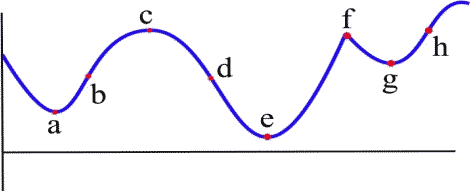
\includegraphics{images/image053.png}
\caption{}
\end{figure}

\begin{longtable}[]{@{}ll@{}}
\toprule
\endhead
\href{section1-2.php}{← Previous Section} & \href{section1-4.php}{Next
Section →}\tabularnewline
\bottomrule
\end{longtable}
